\documentclass[11pt]{article}
% Shared preamble for the notes in this repository. pdfLaTeX, TeX Live 2024 or later.
\usepackage[a4paper,margin=2.6cm]{geometry}
\usepackage[T1]{fontenc}
\usepackage{lmodern}
\usepackage{microtype}
\usepackage{amsmath,amssymb,amsthm}
\usepackage{graphicx}
\usepackage{booktabs}
\usepackage{enumitem}
\usepackage[dvipsnames]{xcolor}
\usepackage[hidelinks]{hyperref}
\hypersetup{colorlinks=true,linkcolor=MidnightBlue,citecolor=MidnightBlue,urlcolor=MidnightBlue}
\graphicspath{{../../figures/}}
\setlist{itemsep=2pt,topsep=4pt}

\newtheorem{theorem}{Theorem}
\newtheorem{proposition}[theorem]{Proposition}
\newtheorem{corollary}[theorem]{Corollary}
\newtheorem{conjecture}[theorem]{Conjecture}
\theoremstyle{definition}
\newtheorem{definition}[theorem]{Definition}
% Reusable derivations, numbered note.k; each note sets \notenumber. Indexed in DERIVATIONS.md.
\newcommand{\notenumber}{0}
\newtheorem{derivation}{Derivation}
\renewcommand{\thederivation}{\notenumber.\arabic{derivation}}
\newtheorem{question}{Question}
\theoremstyle{remark}
\newtheorem{remark}[theorem]{Remark}

\newcommand{\Z}{\mathbb{Z}}
\newcommand{\Q}{\mathbb{Q}}
\newcommand{\R}{\mathbb{R}}
\newcommand{\C}{\mathbb{C}}
\newcommand{\HH}{\mathbb{H}}
\newcommand{\SL}{\mathrm{SL}}
\newcommand{\Gal}{\mathrm{Gal}}
\newcommand{\Hom}{\mathrm{Hom}}
\newcommand{\repo}{\href{https://github.com/rmorleysmith/l-functions-and-physics}{\texttt{l-functions-and-physics}}}
\newcommand{\formal}{\href{https://github.com/rmorleysmith/morley-smith-formal}{\texttt{morley-smith-formal}}}
\newcommand{\script}[1]{\href{https://github.com/rmorleysmith/l-functions-and-physics/blob/main/scripts/#1}{\texttt{scripts/#1}}}
% A path inside the Lean repository; it may break after a slash.
\newcommand{\leanpath}[1]{\nolinkurl{#1}}

% Grades used in every status table.
\newcommand{\gradeLean}{\textsc{lean}}      % proved in Lean 4 with Mathlib
\newcommand{\gradeClassical}{\textsc{classical}}  % a published theorem, cited
\newcommand{\gradeComputed}{\textsc{computed}}    % checked numerically by a script in this repository
\newcommand{\gradeConvention}{\textsc{convention}}  % a choice of units or names
\newcommand{\gradeOpen}{\textsc{open}}      % a question, conjecture or working hypothesis
% The legend printed under every status table.
\newcommand{\gradelegend}{\par\nopagebreak\smallskip\noindent\begin{minipage}{\textwidth}\small
\gradeLean: proved in Lean 4 with Mathlib.
\gradeClassical: a published theorem.
\gradeComputed: checked numerically by a script in the repository \repo.
\gradeConvention: a choice of units or names.
\gradeOpen: a question, conjecture or working hypothesis.
\end{minipage}\par\medskip}
% A plain-language physical reading, placed after each derivation.
\newcommand{\physical}{\paragraph{In physical terms.}}

\renewcommand{\notenumber}{9}

\title{The zeros as energy levels}
\author{Richard Morley-Smith}
\date{Note 09 \quad November 2026}

\begin{document}
\maketitle

\begin{abstract}
\noindent
Read the zeros of the zeta function as the energy levels of a quantum system.
Near $t = 10^6$ we locate the 9511 zeros in a window of length 4990, and an exact count shows that each is simple and on the critical line.
Their mean density is a Weyl term.
Their fluctuations are a sum over the primes: the smoothed density of zeros equals the mean density plus one oscillation for each prime power $p^k$, of frequency $k\log p$, to $2\times10^{-10}$.
This is the form of Gutzwiller's trace formula, with the primes as periodic orbits.
At short range the zeros are observed to repel one another as the eigenvalues of random Hermitian matrices do, the statistics of a quantum system without time-reversal symmetry.
At long range they are more rigid than the random matrices, and the difference is given to $0.002$ by Berry's sum over the prime powers.
The primes themselves are spaced like a Poisson process.
Finally, the zeros of the four $L$-functions of $\Q(\zeta_{12})$, the four orthogonal packets of note~07, are consistent with four independent spectra, as Bogomolny and Leboeuf found for Dirichlet $L$-functions: each repels itself, and zeros of different $L$-functions pass one another freely, as energy levels with different quantum numbers do.
\end{abstract}

\section{The zeros in a window}

Hardy's function $Z(t) = e^{i\theta(t)}\zeta(\tfrac12+it)$ is real, and its sign changes are the zeros of $\zeta$ on the critical line (note~04).

\begin{derivation}[the Riemann--Siegel formula]\label{d:rs}
Let $N = \lfloor\sqrt{t/2\pi}\rfloor$ and $p = \sqrt{t/2\pi} - N$. Then
\[
  Z(t) = 2\sum_{n=1}^{N}\frac{\cos(\theta(t) - t\log n)}{\sqrt n}
  + (-1)^{N-1}\Big(\frac{t}{2\pi}\Big)^{-1/4}\Big[C_0(p) + C_1(p)\Big(\frac{t}{2\pi}\Big)^{-1/2}\Big] + O(t^{-5/4}),
\]
with $C_0(p) = \cos(2\pi(p^2-p-\tfrac1{16}))/\cos(2\pi p)$ and $C_1 = -C_0'''/(96\pi^2)$ \cite{Edwards}.
\end{derivation}

\physical
At height $t$ the function $Z$ is a chord of $\sqrt{t/2\pi}$ pure tones, with frequencies $\log n$ and amplitudes $n^{-1/2}$.
Near $t = 10^6$ there are 398 of them.
The script \script{zeros\_statistics.py} evaluates the formula in bulk; it agrees with a multiprecision evaluation \cite{mpmath} to $2.5\times10^{-9}$.

On the window $995290<t<1000280$ the function $Z$ changes sign 9511 times.
The number of zeros of $\zeta$ in the critical strip between these heights, counted with multiplicity, is $N(1000280)-N(995290) = 9511$, by an independent computation with the mpmath library \cite{mpmath}.
So every zero in the window is simple and lies on the critical line.

\section{The mean density}

\begin{derivation}[Riemann--von Mangoldt]\label{d:mean}
The number of zeros with $0<\gamma\le T$ is
\[
  N(T) = \frac{\theta(T)}{\pi} + 1 + S(T),\qquad \theta(T) = \frac T2\log\frac{T}{2\pi} - \frac T2 - \frac\pi8 + O(1/T),
\]
where $S(T) = \frac1\pi\arg\zeta(\tfrac12+iT) = O(\log T)$ \cite{Edwards}.
The mean density of zeros at height $t$ is $\bar d(t) = \frac{1}{2\pi}\log\frac{t}{2\pi}$.
\end{derivation}

\physical
The smooth part $\theta(T)/\pi + 1 = \frac{T}{2\pi}\big(\log\frac{T}{2\pi}-1\big) + \frac78 + O(1/T)$ is a Weyl term: it counts states by phase-space volume.
Berry and Keating obtained exactly this count, the $\frac78$ included, for the classical Hamiltonian $H = xp$ with a cutoff of one Planck cell \cite{BerryKeating}.
To compare zeros at different heights we unfold them: $x_n = \theta(\gamma_n)/\pi + 1$ has mean spacing one.
Near $t=10^6$ the mean density is $1.906$ zeros per unit of $t$.

\section{The fluctuations are the primes}

\begin{derivation}[the explicit formula as a trace formula]\label{d:trace}
Let $g_\sigma$ be the Gaussian of mean zero, width $\sigma$ and total mass one. For real $E$,
\begin{align*}
  \sum_{\mathrm{Re}\,\gamma>0} g_\sigma(\gamma-E) ={}& \frac{1}{2\pi}\int g_\sigma(r-E)\Big[\mathrm{Re}\,\psi\big(\tfrac14+\tfrac{ir}2\big)-\log\pi\Big]dr\\
  &-\frac1\pi\sum_{n\ge2}\frac{\Lambda(n)}{\sqrt n}\,e^{-\sigma^2(\log n)^2/2}\cos(E\log n) + \epsilon,
\end{align*}
where the sum on the left runs over the zeros $\tfrac12+i\gamma$ of $\zeta$, $\psi = \Gamma'/\Gamma$, and $\epsilon = O_\sigma(e^{-E^2/2\sigma^2})$.
This is Weil's explicit formula with a Gaussian test function \cite{IwaniecKowalski}.
\end{derivation}

\noindent
The first term on the right is the mean density $\bar d(E)$, up to $O(\sigma^2/E^2)$.
The second is a sum over the prime powers $n = p^k$: each contributes an oscillation in $E$ of period $2\pi/(k\log p)$ and amplitude $\log p/(\pi p^{k/2})$, damped by the smoothing.

\physical
The level density of a quantum system is a smooth Weyl term plus one oscillation for each periodic orbit of its classical motion, with the period of the orbit as the frequency of the oscillation: this is Gutzwiller's trace formula \cite{Gutzwiller}.
Derivation~\ref{d:trace} has that form, with the sign of every oscillation reversed: each orbit carries a phase $\pi$ \cite{BerryKeating}.
The zeros are the levels; the periodic orbits are the prime powers $p^k$, the orbit of period $\log p$ traversed $k$ times; and the amplitude $\log p/p^{k/2}$ is that of an unstable orbit \cite{BerryKeating}.
With $\sigma=1$, the script evaluates both sides at 400 energies near $E = 997300$ from the 9511 zeros and from the prime powers below 3000.
They agree to $2.2\times10^{-10}$ (Figure~\ref{fig:trace}).
Landau's formula in note~07 is the same statement read in the other direction.

\begin{figure}[ht]
  \centering
  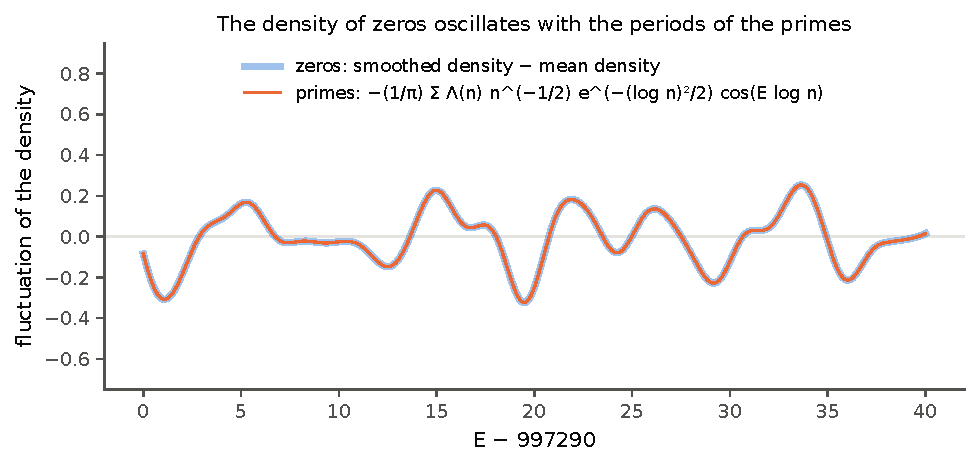
\includegraphics[width=0.92\textwidth]{zeros-trace}
  \caption{The fluctuating part of the density of zeros, smoothed over a width $\sigma=1$ (thick line), and the sum over prime powers (thin line). They coincide.}
  \label{fig:trace}
\end{figure}

\section{Short range: the zeros repel}

\begin{derivation}[Montgomery's pair correlation]\label{d:pair}
For the unfolded zeros, the density of pairs at distance $u$ is conjectured to be
\[
  R_2(u) = 1 - \Big(\frac{\sin\pi u}{\pi u}\Big)^2 .
\]
Montgomery proved this, under the Riemann hypothesis, for test functions whose Fourier transform is supported in $(-1,1)$ \cite{Montgomery}.
It is the pair correlation of the eigenvalues of large random Hermitian matrices, the Gaussian unitary ensemble (GUE) \cite{Mehta}.
\end{derivation}

\physical
The energy levels of a complex quantum system avoid one another.
For generic systems whose classical motion is chaotic, how strongly is conjectured to depend only on a symmetry class: the orthogonal ensemble for systems symmetric under time reversal, and the unitary ensemble for systems that are not \cite{BGS, Mehta}. The Laplacian on the modular surface is an exception: chaotic and symmetric under time reversal, with the level statistics of a Poisson process \cite{ArithmeticChaos}.
The zeros are observed to follow the unitary ensemble, as Odlyzko's computations first showed \cite{Odlyzko}: their statistics are those of a system without time-reversal symmetry.

For the 9511 zeros of the window, the Kolmogorov--Smirnov distance between the nearest-neighbour spacings and the Wigner surmise is $0.015$ for the unitary ensemble, $0.083$ for the orthogonal ensemble and $0.294$ for a Poisson process (Figure~\ref{fig:spacings}, left).
The pair correlation on $0<u<3$ lies at root-mean-square distance $0.042$ from Montgomery's function and $0.344$ from the Poisson value~1 (Figure~\ref{fig:pair}, left).

\begin{figure}[ht]
  \centering
  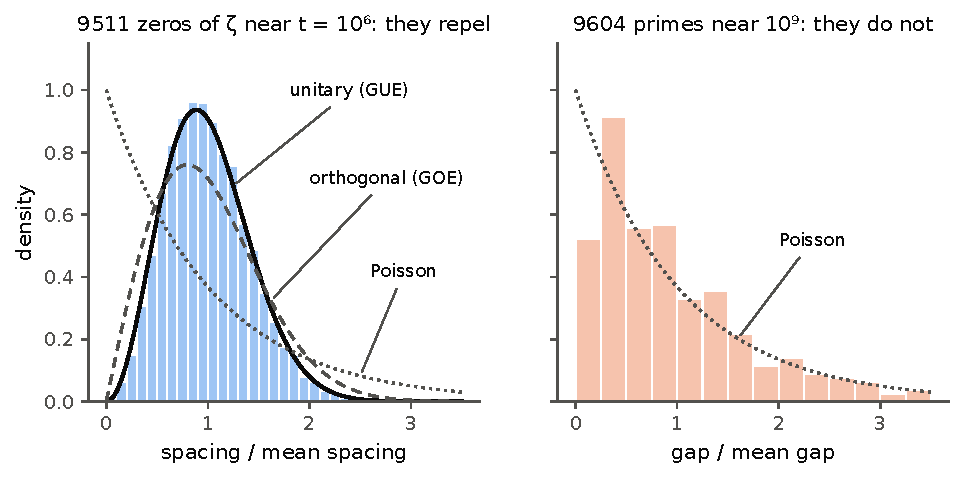
\includegraphics[width=0.92\textwidth]{zeros-spacings}
  \caption{Nearest-neighbour spacings, in units of the mean. Left: the zeros of the window, with the Wigner surmises of the unitary and orthogonal ensembles and the Poisson law. Right: the gaps between the primes in $[10^9, 10^9+2\cdot10^5]$.}
  \label{fig:spacings}
\end{figure}

\section{Long range: the primes set the rigidity}

The number variance $\Sigma^2(L)$ is the variance of the number of unfolded zeros in a window of length $L$.
For a Poisson process it is $L$; for the unitary ensemble it grows only as $\pi^{-2}\log L$ \cite{Mehta}.

\begin{derivation}[Berry's formula]\label{d:berry}
At height $E$, with $X = E/2\pi$,
\[
  \Sigma^2(L) = \frac{2}{\pi^2}\Big[\sum_{p^k<X}\frac{\sin^2\!\big(\pi Lk\log p/\log X\big)}{k^2p^k}
  + \int_1^\infty\frac{\sin^2(\pi L\tau)}{\tau^2}\,d\tau\Big]
\]
in the semiclassical approximation \cite{Berry88}.
\end{derivation}

\noindent
The sum comes from Derivation~\ref{d:mean}: by the Euler product, $S(t) = -\frac1\pi\sum_{p^k}\sin(tk\log p)/(kp^{k/2})$ formally, and the variance of $S(t+\Delta)-S(t)$ over $t$ is $\frac{1}{\pi^2}\sum(1-\cos(\Delta k\log p))/(k^2p^k)$.
Orbits longer than the Heisenberg time, $k\log p>\log X$, act collectively as the random matrices prescribe, which gives the integral.

\physical
Over windows up to about one mean spacing the zeros fluctuate as random matrices do.
Over longer windows they are more rigid, and the extra rigidity is fixed by the shortest periodic orbits, $\log 2$, $\log 3$, $\log 5$: universal statistics at short range, the primes themselves at long range.

The measured variance of the zeros in the window is $0.276$, $0.330$, $0.382$, $0.427$ and $0.441$ at $L = \tfrac12, 1, 2, 4, 6$.
The unitary ensemble gives $0.280$, $0.344$, $0.416$, $0.486$ and $0.527$.
Berry's formula gives $0.275$, $0.329$, $0.382$, $0.427$ and $0.440$, and stays within $0.002$ of the measured values for every $L$ from $0.1$ to $6$ (Figure~\ref{fig:pair}, right).

\begin{figure}[ht]
  \centering
  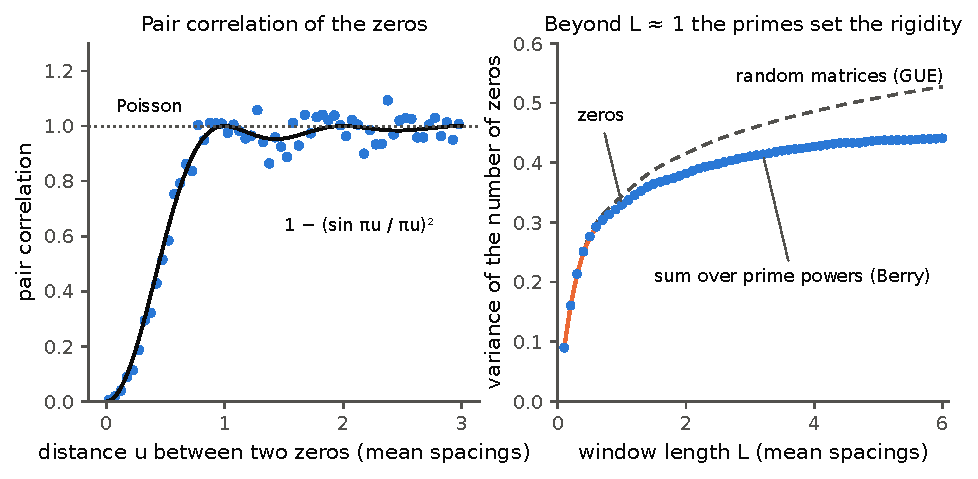
\includegraphics[width=0.92\textwidth]{zeros-pair-variance}
  \caption{Left: the pair correlation of the 9511 zeros, with Montgomery's function. Right: their number variance, with the unitary ensemble (dashed) and Berry's formula (solid).}
  \label{fig:pair}
\end{figure}

\section{The primes, for comparison}

The 9604 primes between $10^9$ and $10^9+2\cdot10^5$, with gaps measured in units of $\log p$, are spaced like a Poisson process (Figure~\ref{fig:spacings}, right), as the prime $k$-tuples conjecture predicts \cite{Gallagher}.

\begin{center}
\small
\begin{tabular}{@{}lcccc@{}}
\toprule
share of spacings in & $[0,\tfrac12)$ & $[\tfrac12,1)$ & $[1,2)$ & $[2,\infty)$\\
\midrule
zeros near $10^6$ & 0.101 & 0.432 & 0.452 & 0.015\\
unitary ensemble & 0.112 & 0.421 & 0.450 & 0.017\\
primes near $10^9$ & 0.352 & 0.275 & 0.249 & 0.124\\
Poisson process & 0.393 & 0.239 & 0.233 & 0.135\\
\bottomrule
\end{tabular}
\end{center}
The zeros' share of small spacings, $0.101$, lies below the ensemble's $0.112$: at this height the zeros are slightly stiffer than the ensemble.

\noindent
The number variance of the primes is $0.79$ and $1.50$ at $L=1$ and $2$, against $0.33$ and $0.38$ for the zeros.
The primes' variance falls below the Poisson values 1 and 2 by a factor of about $\log(x/h)/\log x$, for intervals of length $h$ near $x$.
Goldston and Montgomery showed that, under the Riemann hypothesis, this law for longer intervals is equivalent to the pair correlation of the zeros \cite{GoldstonMontgomery}.

\physical
The impulses of note~07 arrive like raindrops, and their spectrum keeps its distances like the levels of a heavy nucleus.
A random train of impulses has a rigid spectrum.

\section{Four packets, four spectra}

The Dedekind zeta function of $\Q(\zeta_{12})$ is the product of the four $L$-functions of note~01, so its zeros are the union of their zeros.
A fast evaluator for Dirichlet $L$-functions (\script{lfunctions.py}, checked against multiprecision values to $5\times10^{-13}$) finds the zeros below height 600: 341 for $\zeta$, 473 for $\chi_{-4}$, 445 for $\chi_{-3}$ and 577 for $\chi_{12}$, in agreement with the mean counts $340.7$, $472.4$, $444.9$ and $577.0$.

\begin{derivation}[superposing independent spectra]\label{d:super}
Let $E_i(s)$ be the probability that an interval of length $s$ contains no level of the $i$-th spectrum, in units of its own mean spacing.
If the spectra are independent, with relative densities $f_i$, the union has gap probability $E(s) = \prod_i E_i(f_is)$, and its spacings have distribution function $1 + E'(s)$ \cite{BerryRobnik}.
\end{derivation}

\physical
Energy levels that carry different quantum numbers do not repel: they belong to different symmetry sectors and cross freely.
Here the symmetry group is $\Gal(\Q(\zeta_{12})/\Q)$, the Klein four-group of note~01, and its four characters label the sectors.

Each spectrum alone repels itself, and at this low height more strongly than the unitary ensemble: the share of its spacings below half the mean is $0.062$, $0.059$, $0.050$ and $0.064$, against $0.112$ for the ensemble and $0.393$ for a Poisson process, and the Kolmogorov--Smirnov distances to the unitary law are $0.058$, $0.072$, $0.079$ and $0.084$.
The 1836 zeros together are consistent with the spacing law of four independent unitary spectra (distance $0.026$), and they depart from the law of a single spectrum ($0.205$) and from the Poisson law ($0.092$).
Of the 301 spacings of the union below a quarter of the mean, all 301 join zeros of different $L$-functions, as the repulsion within each spectrum requires (Figure~\ref{fig:four}).

\begin{figure}[ht]
  \centering
  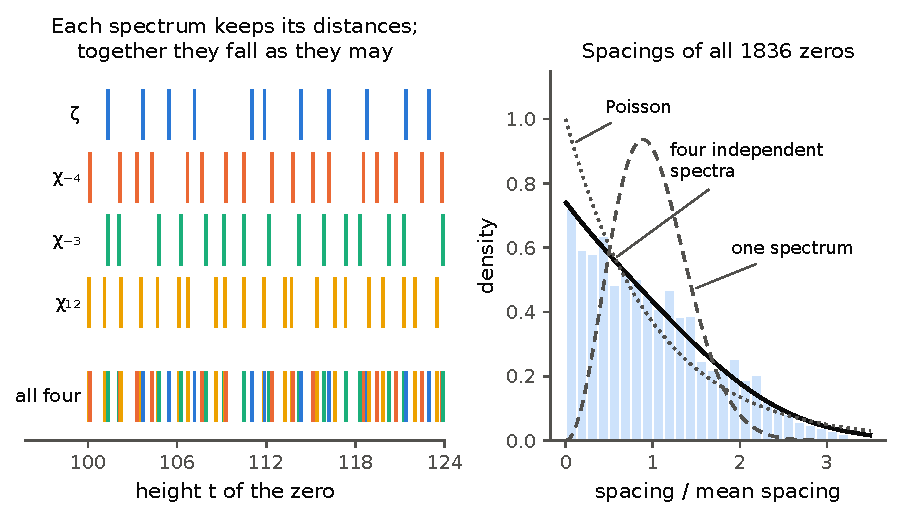
\includegraphics[width=0.92\textwidth]{zeros-four-spectra}
  \caption{Left: the zeros of the four $L$-functions of $\Q(\zeta_{12})$ with $100<t<124$, and their union. Right: the spacings of all 1836 zeros below height 600, with the law of four independent spectra (solid), of one spectrum (dashed) and of a Poisson process (dotted).}
  \label{fig:four}
\end{figure}

\begin{conjecture}[Bogomolny and Leboeuf \cite{BogomolnyLeboeuf}]\label{conj:indep}
The zeros of different Dirichlet $L$-functions are statistically independent.
In particular the four $L$-functions of $\Q(\zeta_{12})$, the orthogonal packets of note~07, have independent spectra.
\end{conjecture}

\noindent
Bogomolny and Leboeuf derive the statement from the Hardy--Littlewood conjecture on prime pairs and test it numerically; the computation above is a check of it for the four characters modulo 12.

\section{Questions}

The Hilbert--P\'olya proposal is that the zeros are the eigenvalues of a self-adjoint operator, which would place them on the critical line.
The statistics above say what kind of system it would be: quantum, classically chaotic, without time-reversal symmetry, with periodic orbits of periods $\log p$ \cite{BerryKeating}.

\begin{question}
Is there a physical system whose energy levels are the zeros of $\zeta$, or of the Dedekind zeta function of $\Q(\zeta_{12})$ with its four symmetry sectors?
\end{question}

\begin{question}
The unitary statistics express the absence of time-reversal symmetry.
Time reversal and parity are different symmetries: a magnetic field breaks the first and not the second.
Would a system whose levels are the zeros also break parity, as the weak interaction does?
\end{question}

\section*{Status of the statements}

\begin{center}
\small
\begin{tabular}{@{}p{0.62\textwidth}l@{}}
\toprule
Statement & Grade\\
\midrule
Derivations~\ref{d:rs}--\ref{d:trace}; Derivation~\ref{d:super} & \gradeClassical\\
All 9511 zeros of the window simple and on the critical line & \gradeComputed\\
Trace formula at 400 energies, to $2.2\times10^{-10}$ & \gradeComputed\\
Pair correlation in general; GUE statistics of the zeros & \gradeOpen; evidence \gradeComputed\\
Berry's semiclassical formula; agreement to $0.002$ for $0.1\le L\le6$ & \gradeOpen; \gradeComputed\\
Primes near $10^9$ against a Poisson process & \gradeComputed\\
The four spectra: counts, self-repulsion, the union consistent with four independent spectra & \gradeComputed\\
Conjecture~\ref{conj:indep}; Questions 1 and 2; the Riemann hypothesis & \gradeOpen\\
\bottomrule
\end{tabular}
\end{center}
\gradelegend

\begin{thebibliography}{99}
\bibitem{Berry88} M.~V. Berry, Semiclassical formula for the number variance of the Riemann zeros, \emph{Nonlinearity} 1 (1988), 399--407.
\bibitem{BerryKeating} M.~V. Berry and J.~P. Keating, The Riemann zeros and eigenvalue asymptotics, \emph{SIAM Rev.} 41 (1999), 236--266.
\bibitem{BerryRobnik} M.~V. Berry and M.~Robnik, Semiclassical level spacings when regular and chaotic orbits coexist, \emph{J. Phys. A} 17 (1984), 2413--2421.
\bibitem{ArithmeticChaos} E.~B. Bogomolny, B.~Georgeot, M.-J. Giannoni and C.~Schmit, Chaotic billiards generated by arithmetic groups, \emph{Phys. Rev. Lett.} 69 (1992), 1477--1480.
\bibitem{BogomolnyLeboeuf} E.~Bogomolny and P.~Leboeuf, Statistical properties of the zeros of zeta functions: beyond the Riemann case, \emph{Nonlinearity} 7 (1994), 1155--1167.
\bibitem{BGS} O.~Bohigas, M.-J. Giannoni and C.~Schmit, Characterization of chaotic quantum spectra and universality of level fluctuation laws, \emph{Phys. Rev. Lett.} 52 (1984), 1--4.
\bibitem{Edwards} H.~M. Edwards, \emph{Riemann's Zeta Function}, Academic Press, 1974.
\bibitem{Gallagher} P.~X. Gallagher, On the distribution of primes in short intervals, \emph{Mathematika} 23 (1976), 4--9.
\bibitem{GoldstonMontgomery} D.~A. Goldston and H.~L. Montgomery, Pair correlation of zeros and primes in short intervals, in \emph{Analytic Number Theory and Diophantine Problems}, Birkh\"auser, 1987, 183--203.
\bibitem{Gutzwiller} M.~C. Gutzwiller, \emph{Chaos in Classical and Quantum Mechanics}, Springer, 1990.
\bibitem{IwaniecKowalski} H.~Iwaniec and E.~Kowalski, \emph{Analytic Number Theory}, American Mathematical Society, 2004.
\bibitem{Mehta} M.~L. Mehta, \emph{Random Matrices}, 3rd ed., Elsevier, 2004.
\bibitem{Montgomery} H.~L. Montgomery, The pair correlation of zeros of the zeta function, in \emph{Analytic Number Theory}, Proc. Sympos. Pure Math. 24, American Mathematical Society, 1973, 181--193.
\bibitem{mpmath} The mpmath development team, \emph{mpmath: a Python library for arbitrary-precision floating-point arithmetic}, version 1.4.1, \url{https://mpmath.org}.
\bibitem{Odlyzko} A.~M. Odlyzko, On the distribution of spacings between zeros of the zeta function, \emph{Math. Comp.} 48 (1987), 273--308.
\end{thebibliography}

\end{document}
